\documentclass[aspectratio=169]{beamer}

\usepackage{fontspec}
\usepackage{microtype}
\usepackage{fontawesome}

\hypersetup{
    colorlinks,
    linkcolor=red,
    pdftitle={Dark Corner of STL},
    pdfpagemode=FullScreen,
    }

\setmonofont{JetBrainsMono}[
    Path=./static/fonts/jetbrains/,
    Scale=0.85,
    Extension = .ttf,
    UprightFont=*-Regular,
    BoldFont=*-Bold,
    ItalicFont=*-Italic,
    BoldItalicFont=*-BoldItalic
    ]
    
\setsansfont{Asap}[
    Path=./static/fonts/asap/,
    Scale=0.9,
    Extension = .ttf,
    UprightFont=*-Regular,
    BoldFont=*-Bold,
    ItalicFont=*-Italic,
    BoldItalicFont=*-BoldItalic
    ]
    
\usepackage[newfloat=true]{minted}
\usemintedstyle{xcode}
\beamertemplatenavigationsymbolsempty

\setbeamertemplate{footline}{\begin{center}\quad\insertframenumber\strut\quad\end{center}}
\setbeamerfont{footline}{size=\large}


%\setbeameroption{hide notes} % Only slides
%\setbeameroption{show only notes} % Only notes
%\setbeameroption{show notes on second screen=left}


\title{The Dark Corner of STL: MinMax Algorithms}
\author{Šimon Tóth}

\begin{document}

{
\usebackgroundtemplate{
\includegraphics[width=\paperwidth]{static/first-slide.png}}
\begin{frame}[plain]
\end{frame}
}

%\frame{\titlepage}

\begin{frame}{Permanent link}
    \begin{center}
        \Large\href{https://github.com/HappyCerberus/cppcon22-talk}{https://github.com/HappyCerberus/cppcon22-talk}\\
        
\includegraphics[width=.4\textwidth]{static/qr-code.png}
    \end{center}
\end{frame}

\begin{frame}{Prior art}
Walter E. Brown - Correctly calculating min, max and more
\begin{itemize}
    \item how to correctly implement min, max algorithms
    \item nuances of less than comparison
\end{itemize}
\end{frame}

%\begin{frame}{}
%\Huge\begin{center}The Dark Corner of STL\\\Large MinMax Algorithms\\\vspace{2em}\small Šimon Tóth\end{center}\vspace{2em}\small
%
%\begin{columns}
%    \begin{column}{0.7\textwidth}\end{column}
%    \begin{column}{0.3\textwidth}
%        \begin{columns}[onlytextwidth,t]
%            \begin{column}{0.1\textwidth}
%                \faTwitter\\ \faLinkedin\\ \faGithub
%            \end{column}
%            \begin{column}{0.85\textwidth}
%                \href{https://twitter.com/SimonToth83}{SimonToth83}\\
%                \href{https://cz.linkedin.com/in/simontoth}{SimonToth}\\
%                \href{https://github.com/HappyCerberus}{HappyCerberus}
%            \end{column}
%        \end{columns}
%    \end{column}
%\end{columns}
%\end{frame}

\begin{frame}{}
    \begin{columns}
        \begin{column}{0.3\textwidth}
            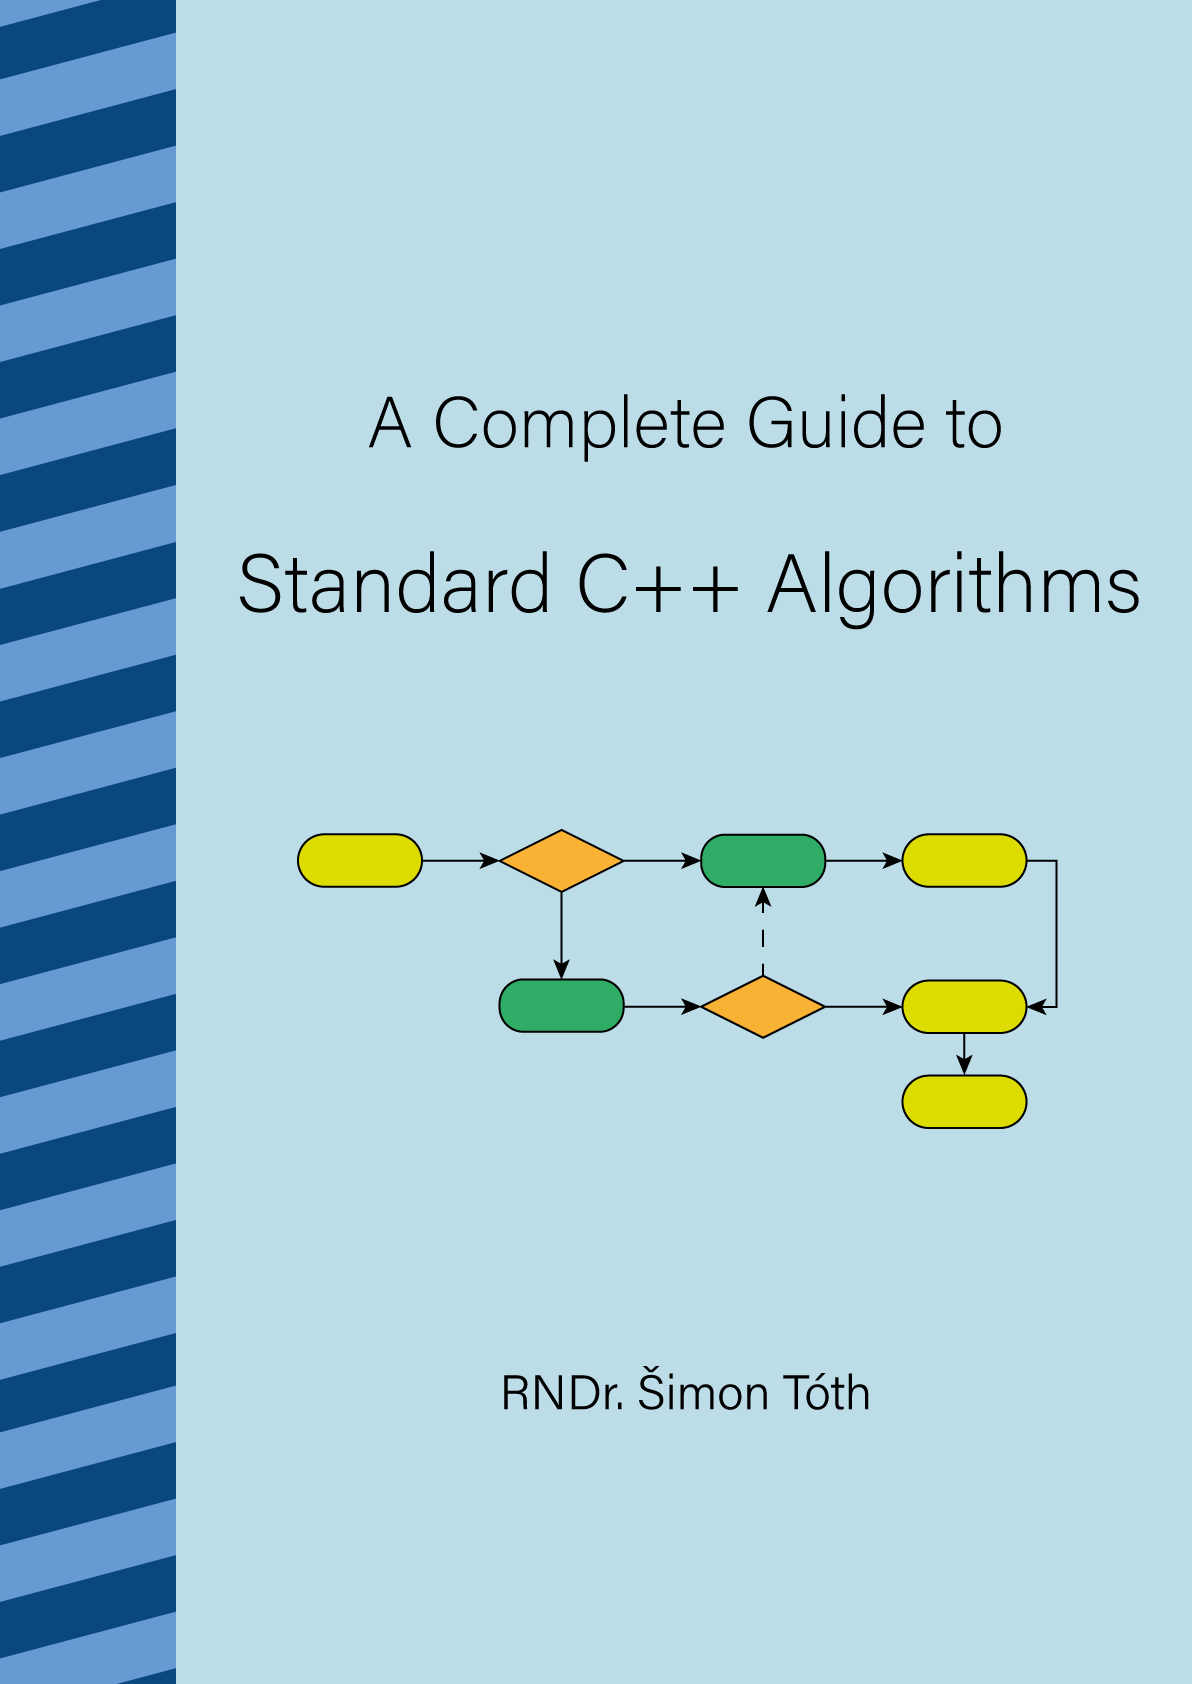
\includegraphics[height=0.8\textheight]{static/book_cover.png}
        \end{column}
        \begin{column}{0.6\textwidth}
            \begin{itemize}
                \item Free on GitHub:\\
                    \href{https://github.com/HappyCerberus/book-cpp-algorithms}{HappyCerberus/book-cpp-algorithms}
                \item Donate to EFF on LeanPub:\\
                    \href{https://leanpub.com/cpp-algorithms-guide}{leanpub.com/cpp-algorithms-guide}
            \end{itemize}
        \end{column}
    \end{columns}
\end{frame}

\begin{frame}[c]
\begin{center}
    \huge How hard is it to call \texttt{std::min}?
\end{center}
\end{frame}

\begin{frame}[fragile,c]
\begin{minted}[escapeinside=||]{cpp}
auto min = std::min(1, 2);

|\pause|auto max = std::max(1, 2);

|\pause|auto clamped = std::clamp(0, 1, 2);

|\pause|auto minmax = std::minmax(1, 2);
\end{minted}
\end{frame}

\begin{frame}[fragile]{}
\begin{small}
\begin{minted}{cpp}
template< class T >
const T& min( const T& a, const T& b );

template< class T >
const T& max( const T& a, const T& b );

template< class T >
const T& clamp( const T& v, const T& lo, const T& hi );

template< class T >
std::pair<const T&,const T&> minmax( const T& a, const T& b );
\end{minted}
\end{small}
\end{frame}

\begin{frame}[fragile]{}
\begin{minted}[escapeinside=||]{cpp}
std::pair<const int&, const int&> a = std::minmax(1, 2);
// a.first, a.second are now dangling references

|\pause|const int& b = std::min(1, 2);
// b is now a dangling reference

|\pause|auto c = std::min(1, 2);
// decltype(c) == int

|\pause|auto d = std::minmax(1, 2);
// decltype(d) == std::pair<const int&, const int&>
\end{minted}
\end{frame}

\begin{frame}[fragile]{}
\begin{minted}[escapeinside=||]{cpp}
auto [x, y] = std::minmax(1, 2);
// decltype(x) == const int&, decltype(y) == const int&

|\pause|std::pair<int, int> a = std::minmax(1, 2);
// OK, capture by-copy
\end{minted}
\end{frame}

\begin{frame}[fragile,c]
\mintinline{text}{g++ sample.cc -fsanitize=address -g && ./a.out}
\vspace{2em}
\begin{tiny}
\begin{minted}{text}
=================================================================
==119==ERROR: AddressSanitizer: stack-use-after-scope on address 0x7ffccaf6cd10
    at pc 0x55df7a7364b0 bp 0x7ffccaf6cce0 sp 0x7ffccaf6ccd0
READ of size 4 at 0x7ffccaf6cd10 thread T0
    #0 0x55df7a7364af in main /home/simon/main.cpp:7
    #1 0x7f61baf18d8f  (/lib/x86_64-linux-gnu/libc.so.6+0x29d8f)
    #2 0x7f61baf18e3f in __libc_start_main (/lib/x86_64-linux-gnu/libc.so.6+0x29e3f)
    #3 0x55df7a736264 in _start (/home/simon/a.out+0x1264)

Address 0x7ffccaf6cd10 is located in stack of thread T0 at offset 32 in frame
    #0 0x55df7a736338 in main /home/simon/main.cpp:5
\end{minted}
\end{tiny}
\end{frame}

\begin{frame}{Variants}
\begin{itemize}
    \item \pause (C++20) range versions have identical behaviour\newline\\
    \small\mintinline{cpp}{range_value_t<R> min(R&& r, Comp comp, Proj proj);}\newline\\
    \item \pause(C++14) \mintinline{cpp}{initializer_list} variants return by value
\end{itemize}
\end{frame}

\begin{frame}[fragile]{}
\begin{minted}[escapeinside=||]{cpp}
auto x = std::min({1, 2});
// OK, decltype(x) == int

auto y = std::minmax({1, 2});
// OK, decltype(y) == std::pair<int,int>

|\pause|const int& z = std::min({1, 2});
// OK, lifetime extension

\end{minted}
\end{frame}

\begin{frame}[fragile]{}
\begin{minted}[escapeinside=||]{cpp}
auto x = std::min({MoveOnly{}, MoveOnly{}});
// Wouldn't compile, can't move-out-of initializer_list.

|\pause|ExpensiveToCopy a, b;
auto y = std::min({ a, b });
// 3x copy

|\pause|auto z = std::min({ExpensiveToCopy{}, ExpensiveToCopy{}});
// 1x copy since C++17 (copy-initialization from prvalue)
\end{minted}
\end{frame}

\begin{frame}[fragile]{const correctness}
\pause\begin{minted}[escapeinside=||]{cpp}
MyType a, b;

if (b < a) {
    b.do_something();
} else {
    a.do_something();
}
\end{minted}
\end{frame}

\begin{frame}[fragile]{const correctness}
\begin{minted}[escapeinside=||]{cpp}
MyType a, b;

std::min(a,b).do_something();

|\pause|const_cast<MyType&>(std::min(a,b)).do_something();
\end{minted}
\end{frame}

\begin{frame}[fragile]{const correctness}
\begin{minted}[escapeinside=||]{cpp}
const MyType a, b;

const_cast<MyType&>(std::min(a,b)).do_something();
// Undefined Behaviour (if do_something mutates state)
\end{minted}
\end{frame}


\begin{frame}[c]{}
\center{\huge{Can we fix it?}}
\end{frame}

\begin{frame}{Target behaviour}
\begin{itemize}
    \item<1-> remove the need for \mintinline{cpp}{const_cast}\\
    \small{\textit{when invoked with two mutable lvalue arguments\\
    \hspace{2em}$\Rightarrow$ return (pair of) lvalue reference}}
    \item<2-> remove the potential for dangling reference\\
    \small{\textit{when either argument is prvalue\\
    \hspace{2em}$\Rightarrow$ return by value}}
    \item<3-> avoid excessive copies\\
    \small{\textit{only copy when returning by value\\
    and only the arguments that are returned}}
\end{itemize}
\end{frame}

\begin{frame}[fragile]{}
\begin{flushright}\small\href{https://godbolt.org/z/ejvKx8YEh}{https://godbolt.org/z/ejvKx8YEh}\end{flushright}
\begin{minted}[escapeinside=||]{cpp}
// 1.
template <typename T> const T& min(const T& a, const T& b);

|\pause|// 2.
template <typename T> T& min(T& a, T& b);

|\pause|// 3.
template <typename T> T min(T&& a, const T& b);

// 4.
template <typename T> T min(const T& a, T&& b);

|\pause|// 5.
template <typename T> T min(T&& a, T&& b);
\end{minted}
\end{frame}

\begin{frame}[fragile]{}
\begin{minted}[escapeinside=||]{cpp}
int x = 1, y = 2;

int &a = min(x,y);
|\pause|// OK (lvalue, lvalue) -> lvalue

|\pause|const int &b = min(10,20);
|\pause|// OK, lifetime extension

|\pause|auto c = minmax(10,20);
|\pause|// OK, decltype(c) == std::pair<int,int>
\end{minted}
\end{frame}

\begin{frame}[fragile]{}
Thanks to Luke D'Alessandro!
%\href{https://godbolt.org/z/fc5P3eKnG}{https://godbolt.org/z/fc5P3eKnG}
\href{https://godbolt.org/z/6qdGvczz3}{https://godbolt.org/z/6qdGvczz3}
\begin{minted}[escapeinside=||]{cpp}
|\pause|// 1.
auto min(auto& x, auto& y) -> auto& {
    return y < x ? y : x;
}

|\pause|// 2.
auto min(auto&& x, auto&& y) {
    return y < x ? y : x;
}
\end{minted}
\end{frame}

\begin{frame}[fragile]{}
\begin{small}
\begin{minted}[escapeinside=||]{cpp}
// 1.
auto min(auto& x, auto& y) -> auto& {
    if (y < x)
        return y;
    return x;
}

|\pause|auto min(auto& x, auto& y)
    -> std::common_reference_t<decltype(x),decltype(y)> {
    if (y < x)
        return y;
    return x;
}
\end{minted}
\end{small}
\end{frame}

\begin{frame}[fragile]{}
\begin{small}
\begin{minted}[escapeinside=||]{cpp}
// 1.
auto min(auto& x, auto& y) -> auto& {
    return y < x ? y : x;
}

|\pause|auto min(auto& x, auto& y) -> auto&
requires std::is_same_v<std::remove_cvref_t<decltype(x)>, 
                        std::remove_cvref_t<decltype(y)>> {
    return y < x ? y : x;
}
\end{minted}
\end{small}
\end{frame}

\begin{frame}[fragile]{}
\begin{small}
\begin{minted}[escapeinside=||]{cpp}
// 2.
auto min(auto&& x, auto&& y) {
    return y < x ? y : x;
}

|\pause|auto min(auto&& x, auto&& y) {
    return y < x ? std::forward<decltype(y)>(y) : 
                   std::forward<decltype(x)>(x);
}
\end{minted}
\end{small}
\end{frame}

\begin{frame}[fragile]{}
\begin{small}
\begin{minted}{cpp}
// Min - rvalue variant
constexpr auto min(auto&& x, auto&& y)
    requires std::is_same_v<std::remove_cvref_t<decltype(x)>, 
                            std::remove_cvref_t<decltype(y)>>
{
    return y < x ? std::forward<decltype(y)>(y) : 
                   std::forward<decltype(x)>(x);
}

// Min - lvalue variant
constexpr auto min(auto& x, auto& y) -> auto&
    requires std::is_same_v<std::remove_cvref_t<decltype(x)>, 
                            std::remove_cvref_t<decltype(y)>>
{
    return y < x ? y : x;
}
\end{minted}
\end{small}
\end{frame}

%\begin{frame}[fragile]{}
%\begin{small}
%\begin{minted}{cpp}
%// MinMax - rvalue variant
%constexpr auto minmax(auto&& x, auto&& y)
%    requires std::is_same_v<std::remove_cvref_t<decltype(x)>, 
%                            std::remove_cvref_t<decltype(y)>>
%{
%    return y < x ? 
%        std::pair{std::forward<decltype(y)>(y), 
%                  std::forward<decltype(x)>(x)} :
%        std::pair{std::forward<decltype(x)>(x), 
%                  std::forward<decltype(y)>(y)};
%}
%\end{minted}
%\end{small}
%\end{frame}

\begin{frame}[fragile]{}
\begin{small}
\begin{minted}{cpp}
// MinMax - lvalue variant
constexpr auto minmax(auto& x, auto& y)
    requires std::is_same_v<std::remove_cvref_t<decltype(x)>, 
                            std::remove_cvref_t<decltype(y)>>
{
    using ref = std::common_reference_t<decltype(x),decltype(y)>;
    return y < x ? std::pair<ref,ref>{y,x} : 
                   std::pair<ref,ref>{x,y};
}
\end{minted}
\end{small}
\end{frame}

\begin{frame}[c]
\begin{center}
    \huge How hard is it to call \texttt{std::min}?\\\vspace{1em}
    \pause
\includegraphics[height=0.6\textheight]{static/warning.png}
\end{center}
\end{frame}

\begin{frame}{}
    \begin{columns}
        \begin{column}{0.3\textwidth}
            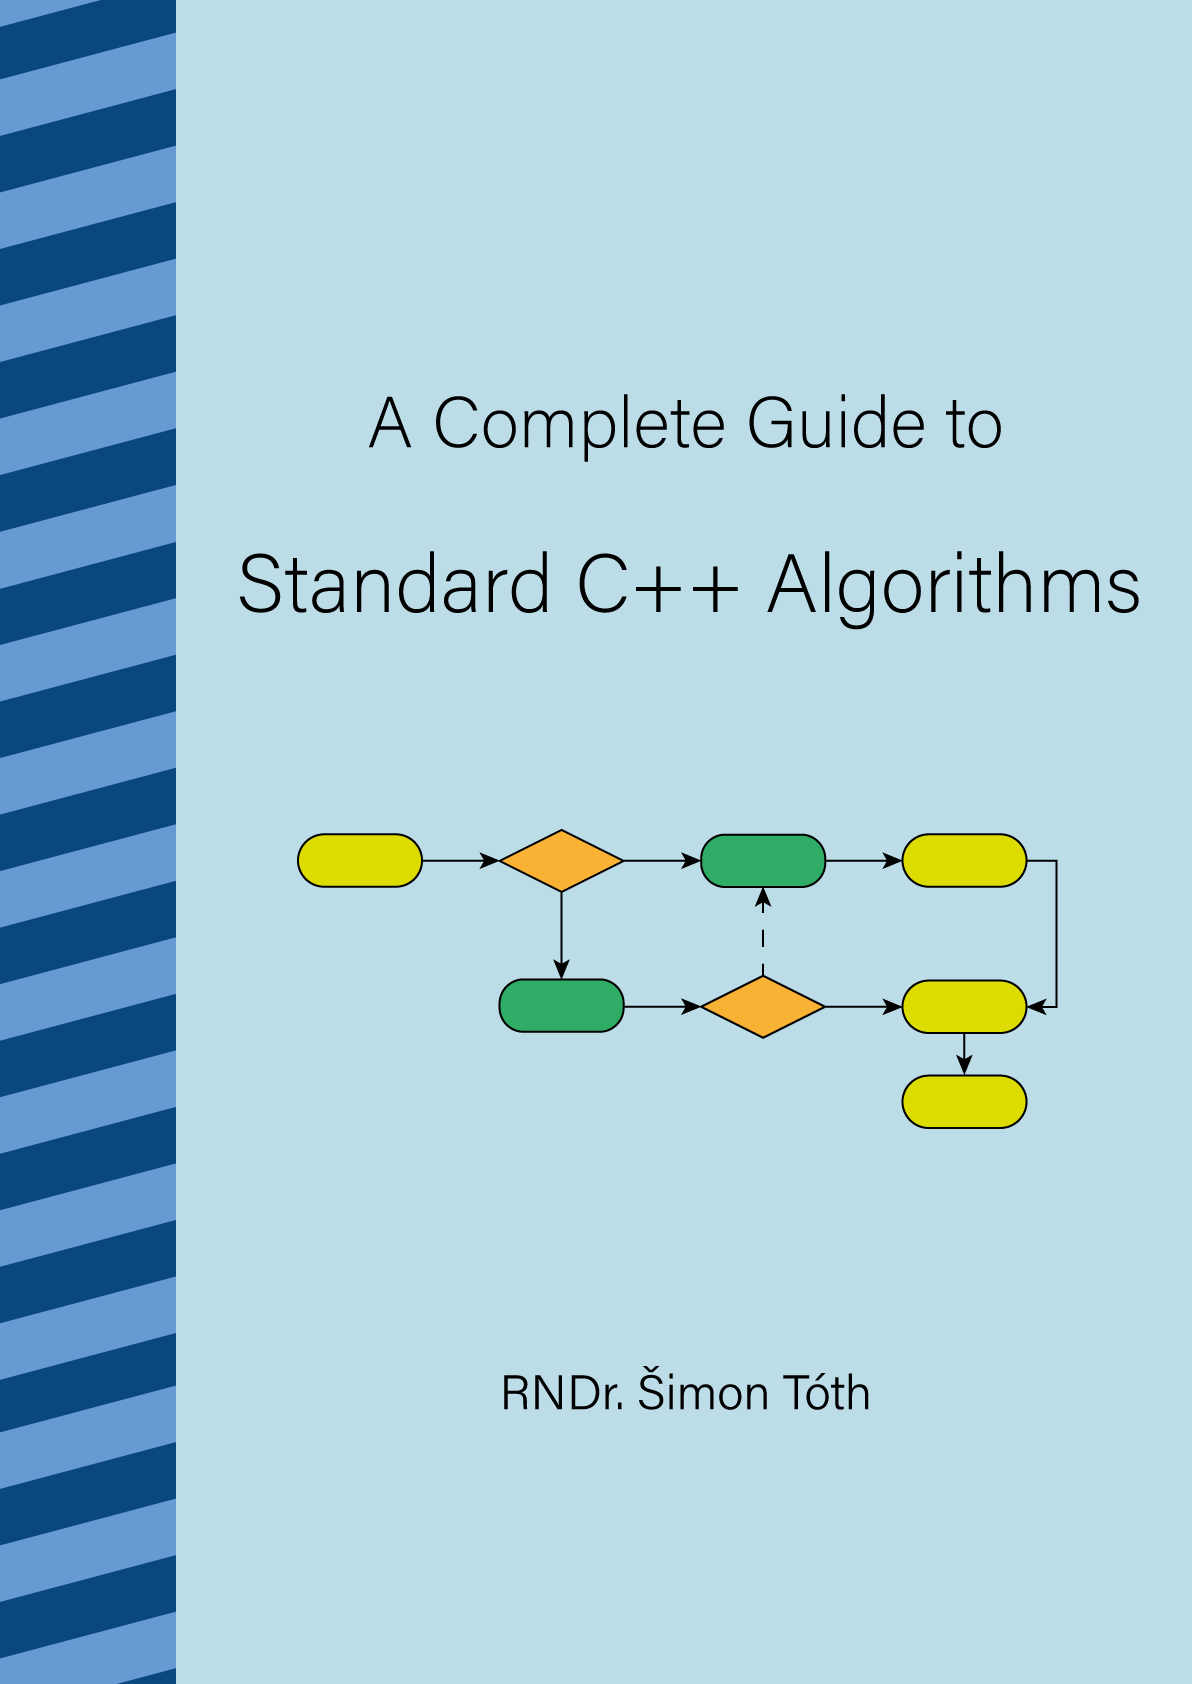
\includegraphics[height=0.8\textheight]{static/book_cover.png}
        \end{column}
        \begin{column}{0.6\textwidth}
            \begin{itemize}
                \item Free on GitHub:\\
                    \href{https://github.com/HappyCerberus/book-cpp-algorithms}{HappyCerberus/book-cpp-algorithms}
                \item Donate to EFF on LeanPub:\\
                    \href{https://leanpub.com/cpp-algorithms-guide}{leanpub.com/cpp-algorithms-guide}
            \end{itemize}
        \end{column}
    \end{columns}
\end{frame}

\begin{frame}[fragile]{References and links}
    \begin{itemize}
        \item \href{https://godbolt.org/z/5Tv3zfTPP}{Demo of \mintinline{cpp}{std::minmax} with \mintinline{text}{-fsanitize=address}}
        \item \href{https://en.cppreference.com/w/cpp/language/lifetime#Temporary_object_lifetime}{Temporary object lifetime}
        \item \href{https://en.cppreference.com/w/cpp/language/template_argument_deduction#auto_type_deduction}{\mintinline{cpp}{auto} type deduction}
        \item \href{https://en.cppreference.com/w/cpp/utility/initializer_list}{\mintinline{cpp}{std::initializer_list}}
        \item \href{https://en.cppreference.com/w/cpp/language/const_cast}{\mintinline{cpp}{const_cast}}
        \item \href{https://en.cppreference.com/w/cpp/types/common_reference}{\mintinline{cpp}{std::common_reference}}
        \item \href{https://en.cppreference.com/w/cpp/language/constraints#Requires_clauses}{\mintinline{cpp}{requires} clause}
        \item \href{https://en.cppreference.com/w/cpp/types/is_same}{\mintinline{cpp}{std::is_same}}
        \item \href{https://godbolt.org/z/1vGxe4Yqr}{All combinations for  \mintinline{cpp}{std::common_reference_t}}
        \item \href{https://godbolt.org/z/ejvKx8YEh}{brute-force "solution"}
        \item \href{https://godbolt.org/z/6qdGvczz3}{C++20 "solution"}
        \item \href{https://godbolt.org/z/8x8sPYG4v}{variadric version of min}
    \end{itemize}
\end{frame}

\begin{frame}[c]{}
    \center{\huge{Bonus slides}}
\end{frame}

\begin{frame}[fragile]{Performance-first alternative}
\begin{minted}{cpp}
auto min(auto& x, auto& y) -> auto& {
    return y < x ? y : x;
}

// Prohibit rvalues altogether.
auto min(auto&&, auto&&) = delete;
\end{minted}
\end{frame}

\begin{frame}[fragile]{clamp}
\begin{small}
\begin{minted}{cpp}
constexpr auto clamp(auto& v, auto& lo, auto& hi) 
    -> std::common_reference_t<decltype(v),decltype(lo),decltype(hi)>

requires
    std::is_same_v<std::remove_cvref_t<decltype(lo)>,
        std::remove_cvref_t<decltype(hi)>> &&
    std::is_same_v<std::remove_cvref_t<decltype(v)>,
        std::remove_cvref_t<decltype(hi)>>

{
    if (v < lo) return lo;
    if (v > hi) return hi;
    return v;
}
\end{minted}
\end{small}
\end{frame}

\end{document}